% generated by experiments/make_figures.py from results/tpch_sf0.1.json and tpch_bandwidth.json
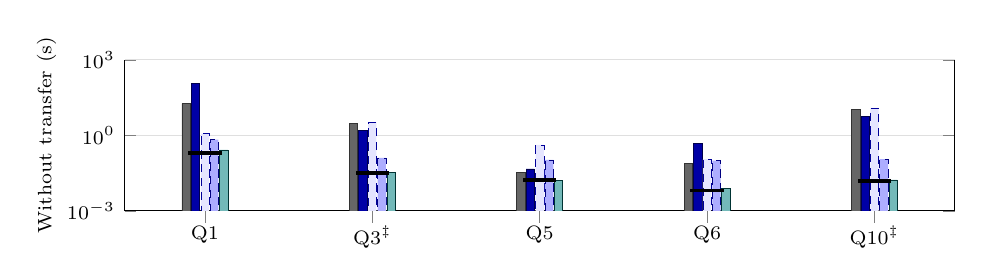
\begin{tikzpicture}
\begin{axis}[
  ybar=0.4pt, ymode=log, log origin=infty, width=\columnwidth, height=3.5cm,
  bar width=3pt, enlarge x limits=0.12, ymin=0.001, ymax=1000,
  symbolic x coords={Q1,Q3,Q5,Q6,Q10}, xtick=data,
  xticklabels={Q1,Q3$^\ddagger$,Q5,Q6,Q10$^\ddagger$},
  tick label style={font=\scriptsize}, label style={font=\scriptsize},
  xticklabel style={align=center, inner sep=1pt},
  ylabel={Without transfer (s)}, ylabel shift=-3pt, ymajorgrids, grid style={gray!25}, axis x line*=bottom,
  legend style={font=\scriptsize, draw=none, fill=none, legend columns=2, /tikz/every even column/.append style={column sep=4pt}},
  legend image code/.code={\draw[#1] (0cm,-0.08cm) rectangle (0.22cm,0.12cm);}, legend cell align=left,
  legend to name=tpchleg,
]
\addplot[fill=black!60, draw=black!80, line width=0.2pt, bar shift=-6.80pt] coordinates {(Q1,18.1489) (Q3,3.09726) (Q5,0.0337263) (Q6,0.0770615) (Q10,10.9153)};
\addplot[fill=blue!65!black, draw=blue!30!black, line width=0.2pt, bar shift=-3.40pt] coordinates {(Q1,120.167) (Q3,1.6154) (Q5,0.0467048) (Q6,0.476521) (Q10,5.48746)};
\addplot[fill=blue!10, draw=blue!60!black, densely dashed, line width=0.2pt, bar shift=0.00pt] coordinates {(Q1,1.17989) (Q3,3.22058) (Q5,0.418793) (Q6,0.114379) (Q10,12.476)};
\addplot[fill=blue!32, draw=blue!50!black, densely dashed, line width=0.2pt, bar shift=3.40pt] coordinates {(Q1,0.68293) (Q3,0.128505) (Q5,0.10665) (Q6,0.0996022) (Q10,0.114517)};
\addplot[fill=teal!55, draw=teal!40!black, line width=0.2pt, bar shift=6.80pt] coordinates {(Q1,0.263185) (Q3,0.03289) (Q5,0.0166315) (Q6,0.00805899) (Q10,0.0170384)};
\addplot[only marks, mark=-, mark size=6pt, line width=1.4pt, black, bar shift=0pt, legend image code/.code={\draw[black, line width=1.4pt] (0cm,0.02cm) -- (0.22cm,0.02cm);}] coordinates {(Q1,0.203725) (Q3,0.0332195) (Q5,0.0163184) (Q6,0.00644167) (Q10,0.0153167)};
\addlegendimage{fill=white, draw=black!60, line width=0.2pt, postaction={pattern=north east lines, pattern color=black!60}}
\legend{{CryptDB, Paillier (non-PQ)},{BFV, one value per ct.$^\ddagger$ (PQ)},{BFV, packed (PQ)},{BFV, packed, client grouping (PQ)},{ASHE (PQ)},{Relational part on DET/OPE (all)},{Transfer to client at 100\,Mbps}}
\end{axis}
\end{tikzpicture}

\begin{tikzpicture}
\begin{axis}[
  ybar=0.4pt, ymode=log, log origin=infty, width=\columnwidth, height=3.1cm,
  bar width=3pt, enlarge x limits=0.12, ymin=0.001, ymax=1000,
  symbolic x coords={Q1,Q3,Q5,Q6,Q10}, xtick=data,
  xticklabels={Q1,Q3$^\ddagger$,Q5,Q6,Q10$^\ddagger$},
  tick label style={font=\scriptsize}, label style={font=\scriptsize},
  xticklabel style={align=center, inner sep=1pt},
  ylabel={With transfer (s)}, ylabel shift=-3pt, ymajorgrids, grid style={gray!25}, axis x line*=bottom,
  legend style={font=\scriptsize, draw=none, fill=none, legend columns=-1, /tikz/every even column/.append style={column sep=4pt}},
  legend image code/.code={\draw[#1] (0cm,-0.08cm) rectangle (0.22cm,0.12cm);}, legend cell align=left,
]
\addplot[fill=black!60, draw=black!80, line width=0.2pt, bar shift=-6.80pt, forget plot, postaction={pattern=north east lines, pattern color=white}] coordinates {(Q1,18.1498) (Q3,3.1435) (Q5,0.0339375) (Q6,0.0771025) (Q10,11.0734)};
\addplot[fill=blue!65!black, draw=blue!30!black, line width=0.2pt, bar shift=-3.40pt, forget plot, postaction={pattern=north east lines, pattern color=white}] coordinates {(Q1,120.829) (Q3,38.9474) (Q5,0.21219) (Q6,0.509617) (Q10,133.27)};
\addplot[fill=blue!10, draw=blue!60!black, densely dashed, line width=0.2pt, bar shift=0.00pt, forget plot, postaction={pattern=north east lines, pattern color=blue!60!black}] coordinates {(Q1,1.84181) (Q3,40.5525) (Q5,0.584277) (Q6,0.147475) (Q10,140.258)};
\addplot[fill=blue!32, draw=blue!50!black, densely dashed, line width=0.2pt, bar shift=3.40pt, forget plot, postaction={pattern=north east lines, pattern color=blue!60!black}] coordinates {(Q1,12.9283) (Q3,2.57762) (Q5,2.52264) (Q6,2.54868) (Q10,2.56362)};
\addplot[fill=teal!55, draw=teal!40!black, line width=0.2pt, bar shift=6.80pt, forget plot, postaction={pattern=north east lines, pattern color=white}] coordinates {(Q1,0.281895) (Q3,0.0340662) (Q5,0.0167785) (Q6,0.00983891) (Q10,0.0214351)};
\addplot[fill=black!60, draw=black!80, line width=0.2pt, bar shift=-6.80pt] coordinates {(Q1,18.1489) (Q3,3.09726) (Q5,0.0337263) (Q6,0.0770615) (Q10,10.9153)};
\addplot[fill=blue!65!black, draw=blue!30!black, line width=0.2pt, bar shift=-3.40pt] coordinates {(Q1,120.167) (Q3,1.6154) (Q5,0.0467048) (Q6,0.476521) (Q10,5.48746)};
\addplot[fill=blue!10, draw=blue!60!black, densely dashed, line width=0.2pt, bar shift=0.00pt] coordinates {(Q1,1.17989) (Q3,3.22058) (Q5,0.418793) (Q6,0.114379) (Q10,12.476)};
\addplot[fill=blue!32, draw=blue!50!black, densely dashed, line width=0.2pt, bar shift=3.40pt] coordinates {(Q1,0.68293) (Q3,0.128505) (Q5,0.10665) (Q6,0.0996022) (Q10,0.114517)};
\addplot[fill=teal!55, draw=teal!40!black, line width=0.2pt, bar shift=6.80pt] coordinates {(Q1,0.263185) (Q3,0.03289) (Q5,0.0166315) (Q6,0.00805899) (Q10,0.0170384)};
\end{axis}
\end{tikzpicture}

{\setlength{\tabcolsep}{2pt}\pgfplotslegendfromname{tpchleg}}
